%\vspace{-4pt}
\subsection{Target Platform}
\label{sec:Platform}

To balance flexibility and efficiency, domain platform includes hardware accelerators (HWACC) and programmable processors (CPU, GPU, DSP), similar to current platforms. However, the number of HWACCs will increase dramatically, where individual HWACCs are less monolithic but smaller and configurable. HWACCs can be composed to accelerate larger kernels (or even applications), e.g. ACC-Rich MPSoCs \cite{cong2014accelerator} and FLP \cite{tabkhi2014function}. 

\begin{figure}[h]
	%\vspace{-4pt}
	\centering
	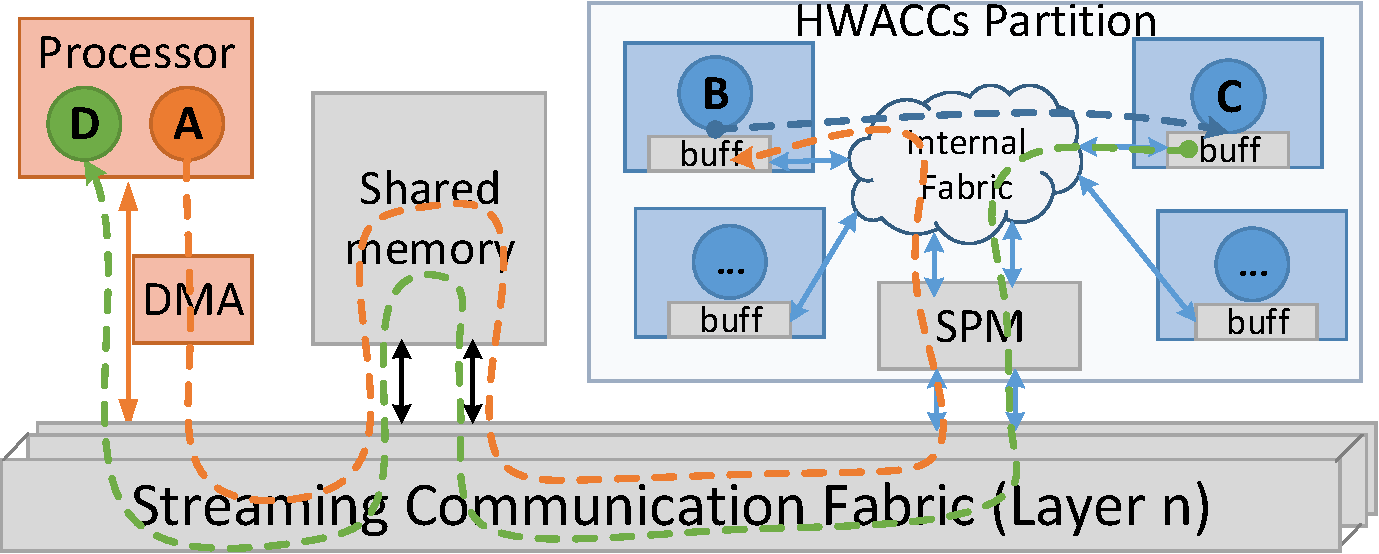
\includegraphics[width=.65\linewidth]{fig/pPlat.pdf}
	%\vspace{-6pt}
	\caption{Target Platform}
	\label{fig:plat}
	%\vspace{-4pt}
\end{figure}

\figref{fig:plat} illustrates the target platform for the context of this work. A streaming application $A$,$B$,$C$,$D$ is mapped across SW and HW. Each HWACC has a dedicated SPM. All HWACCs are aggregated to a HW partition which a shared SPM across all HWACCs. HWACCs can communicate with each other; their communication traffic is hidden from system communication fabric (e.g. $B$, $C$). For simplicity, we assume direct n:n communication within the HW partition. Conversely, HWACCs and SW kernels communicate through the system streaming fabric (e.g. $A$ to $B$, and $C$ to $D$) which results in throughput penalties.


\newtext{Evaluating domain platforms is challenging due to the enormous design space needing to evaluate (a) the performance of each application given allocation and mapping, and (b) systematic aggregation across all applications to determine the platform benefit. For the purpose of this publication, we primarily focus on domain throughput improvement to assess the domain platform benefit. Domain throughput improvement is the average of all applications' throughput improvement each over their own pure SW implementation.} 

\newtext{Evaluating an individual application / platform follows a speed / accuracy trade-off. Transaction Level Models (TLM) can provide a reasonably high accuracy at cost of long simulation times limiting the number of evaluable design points in a given duration. More abstract and dramatically faster evaluation is desired to evaluate many more points at cost of accuracy.} 
~\secref{sec:Ana} and ~\secref{sec:ds} \newtext{propose two approaches and compares them against TLM simulation.}